\documentclass{article}
\usepackage{tikz}
\usetikzlibrary{positioning}
\usetikzlibrary{shapes.geometric}
\usetikzlibrary{shapes.symbols} \usetikzlibrary{shadows}
\usetikzlibrary{arrows}

\pagestyle{empty}

\begin{document}

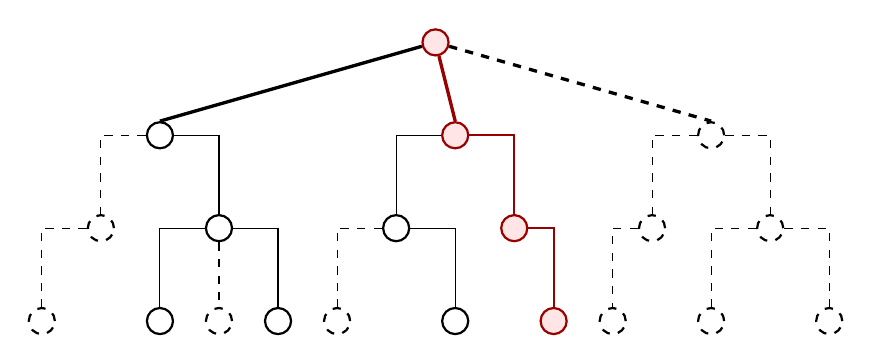
\begin{tikzpicture}
[node/.style={shape=rectangle,draw,thick,below},
 node/.style={shape=ellipse,draw,thick,below},
 selected/.style={draw=red!60!black},
 seledge/.style={selected,thick},
 selnode/.style={red!60!black,selected,fill=red!10!white}]

\draw (0,0) node (root) [node,selnode] {};

\draw [dashed,very thick] (root) -- ++(3.5,-1.0)
	node (s1) [node] {};
\draw [dashed] (s1) -- ++( 0.75,-0) -- ++( 0,-1.0)
	node (s11) [node] {};
\draw [dashed] (s1) -- ++( -0.75,-0) -- ++( 0,-1.0)
	node (s12) [node] {};
\draw [dashed] (s11) -- ++( 0.75,-0) -- ++( 0,-1.0)
	node (s111) [node] {};
\draw [dashed] (s11) -- ++( -0.75,-0) -- ++( 0,-1.0)
	node (s112) [node] {};
\draw [dashed] (s12) -- ++( -0.5,-0) -- ++( 0,-1.0)
	node (s121) [node] {};

\draw [seledge,very thick] (root) -- ++(0.25,-1.0)
	node (s2) [node,selnode] {};
\draw [seledge] (s2) -- ++( 0.75,-0) -- ++( 0,-1.0)
	node (s21) [node,selnode] {};
\draw (s2) -- ++( -0.75,-0) -- ++( 0,-1.0)
	node (s22) [node] {};
\draw [seledge] (s21) -- ++( +0.5,-0) -- ++( 0,-1.0)
	node (s211) [node,selnode] {};
\draw (s22) -- ++( 0.75,-0) -- ++( 0,-1.0)
	node (s221) [node] {};
\draw [dashed] (s22) -- ++( -0.75,-0) -- ++( 0,-1.0)
	node (s222) [node] {};

\draw [very thick] (root) -- ++(-3.5,-1.0)
	node (s3) [node] {};
\draw (s3) -- ++( 0.75,-0) -- ++( 0,-1.0)
	node (s31) [node] {};
\draw [dashed] (s3) -- ++( -0.75,-0) -- ++( 0,-1.0)
	node (s32) [node] {};
\draw (s31) -- ++( 0.75,0) -- ++( 0,-1.0)
	node (s311) [node] {};
\draw [dashed] (s31) -- ++( 0,-1.0)
	node (s312) [node] {};
\draw  (s31) -- ++( -0.75,-0) -- ++( 0,-1.0)
	node (s313) [node] {};
\draw  [dashed] (s32) -- ++( -0.75,-0) -- ++( 0,-1.0)
	node (s311) [node] {};
\end{tikzpicture}
\end{document}
